%\documentclass[twocolumn]{aastex62}
%\documentclass[manuscript]{aastex62}
%\documentclass[preprint]{aastex62}
%\documentclass[preprint2]{aastex62}
%\documentclass{aastex62}
%\documentclass[twocolumn,tighten,longauthor]{aastex62}
%\documentclass[twocolumn,tighten]{aastex62}
%\documentclass[twocolumn,tighten,longauthor,times]{aastex62}
%\documentclass[a4paper]{aastex62}
%\documentclass[a4paper,twoside,10pt]{article}
%\documentclass[preprint,eqsecnum]{aastex62}
%\documentclass[a4paper,preprint]{aastex62}
\documentclass[modern]{aastex62}

%\usepackage{svn}
%\SVNdate $Date: $
%svn propset svn:keywords 'LastChangedDate' main.tex
\usepackage{fancyhdr}
%\usepackage{datetime}
\usepackage{amsmath}                % American Mathematical Society package
\usepackage{amsfonts}               % American Mathematical Society fonts
\usepackage{amssymb}                % American Mathematical Society symbol
\usepackage{amsthm} 
%\usepackage[pdftex]{graphics}
%\usepackage{graphics,epsf}
\usepackage{graphicx}
\usepackage{epsfig}
\usepackage{epstopdf}
\usepackage{figsize}
\usepackage{natbib}
%\bibliographystyle{unsrtnat}
%\bibliographystyle{apj}
%\usepackage[square,numbers]{natbib}
%\bibliographystyle{abbrvnat}

\usepackage{hyperref}
\usepackage{multirow}
\usepackage[para,online,flushleft]{threeparttable}
\usepackage[super]{nth}
\usepackage[inline]{enumitem}

%\usepackage{draftwatermark}
%\SetWatermarkText{DRAFT}
%\SetWatermarkScale{5}

%\usepackage[utf8]{inputenc}
%\usepackage[english]{babel}
 
\usepackage{xcolor}
\usepackage{soul}

\renewcommand{\vec}[1]{\mathbf{#1}}
\newcommand{\fracpartial}[2]{\frac{\partial #1}{\partial #2}}
\newcommand{\Lsun}{\mathrm{L_\odot}}
\newcommand{\ledd}{L_{\mathrm{Edd}}}
\newcommand{\Rsun}{\mathrm{R}_\odot}
\newcommand{\Msun}{\mathrm{M}_\odot}
%\newcommand{\lesim}{{<\atop{\sim}}}
\newcommand{\lesim}{\genfrac{}{}{0pt}{2}{<}{\sim}}
\newcommand{\tred}[1]{\textcolor{red}{#1}}
\newcommand{\tyellow}[1]{\colorbox{yellow}{#1}}
\newcommand{\emphbf}[1]{\textbf{\emph{#1}}}
%\newcommand{\myr}{\mathrm{M_\odot~yr^{-1}}}
\newcommand{\flash}[1]{\textsc{flash}#1}
\newcommand{\radmc}[1]{\textsc{radmc-3d}#1}
\newcommand{\yt}[1]{\texttt{yt}#1}
\newcommand{\visit}[1]{Visit#1}
\newcommand{\python}[1]{Python#1}

\def \kms{~\rm{km~s^{-1}}}
\def \kev{~\rm{keV}}
\def \eV{~\rm{eV}}
\def \cmcub{$\rm{cm}^{-3}$}
\def \msyr{~\rm{M_{\odot}}~\rm{yr^{-1}}}
\def \cm{~\rm{cm}}
\def \s{~\rm{s}}
\def \km{~\rm{km}}
\def \gm{\rm{gm}}
\def \K{~\rm{K}}
\def \g{~\rm{g}}
\def \G{~\rm{G}}
\def \AU{~\rm{AU}}
\def \erg{~\rm{erg}}
\def \yrs{~\rm{yrs}}
\def \yr{~\rm{yr}}
\def \pc{~\rm{pc}}
\def \kpc{~\rm{kpc}}
\def \etc{$\eta$~Car}
\def \days{~\rm{days}}
\def \Jy{~\rm{Jy}}
\def \mum{~\rm{\mu m}}
\def \keV{~\rm{keV}}
\def \astrobj#1{#1}
\def \rmModot{~\rm{M_{\sun}}}
\def \rmRodot{~\rm{R_{\sun}}}
\def \rmLodot{~\rm{L_{\sun}}}
%\def \rmMJ{~\rm{M_J}}
%\def \rmRJ{~\rm{R_J}}

\begin{document}

\title{\LARGE{\textbf{Research Proposal: Simulations of Intermediate Luminosity Optical Transients}}} 
\shorttitle{Research Proposal - Amir Michaelis}
\shortauthors{Research Proposal - Amir Michaelis}


\author[0000-0002-1361-9115]{Amir Michaelis}
%\affil{Department of Physics, Ariel University, Ariel, POB 3, 40700, Israel}
\affil{Advisors: Prof. Gary Gellerman and Dr. Amit Kashi}
\email{amirmi@ariel.ac.il}
%\author[0000-0002-7840-0181]{Advisor: Amit Kashi}
%\affil{Department of Physics, Ariel University, Ariel, POB 3, 40700, Israel}
%\email{kashi@ariel.ac.il}



%\date{\today}

%\submitjournal{ApJ}
%\received{XXX}
%\revised{YYY}
%\accepted{ZZZ}



% \begin{abstract}
% \textbf{We intend to use advanced numerical simulations to reproduce observed features of the transient eruptions, in order to understand the physical processes governing their outbursts.}

% In the past twenty years there many outbursts were observed that first seemed to be supernovae (SN) and after follow-up observation turned to behave differently, and be less luminous. These objects are often called SN imposters. Together with them other types of intermediate luminosity optical transients (ILOTs) were observed and studied as well. On an  energy vs. time diagram, these objects lay on a slated stripe called the optical transient stripe (OTS). Some of them appear different as a result of being oriented differently in space. It was suggested that ILOTs share a similar property – the energy source is gravity that acts in a binary system.

% We adopt the premise that these phenomena can be explained with gravitational binary interaction, and focus on the erupting star V838 Mon, the prototype of a class of erupting objects called luminous red novae (LRNe). These eruptions, as well as many others in the OTS have similar light curves (brightness variability with time), with specific characteristics. The leading model for the eruption mechanism of LRNe is the “mergerburst” model, where a main sequence (MS) star merges with a less dense and lower mass star (a MS or pre-MS star).

% We wish to tie the model and its predictions with the observed light curves. We thus suggest to perform high resolution 3d hydrodynamic simulations of the product of the merger – a MS star surrounded by a thick accretion disk. We will use FLASH hydrodynamic code, a powerful numerical tool in astrophysics, to simulate the physical process of accretion and depletion of the disk. We will later use the radiation transfer code RADMC-3D to simulate the synthetic light curves from different lines of sight, and use them to compare to observed ones.
% \end{abstract}
% \maketitle

% \tableofcontents
% \newpage
%------------------------
\section{Introduction}
%------------------------
Stars that experience transient eruptions are attracting large attention by both observers and theoreticians.
We see a rich variety of luminous transient systems.
In addition to the classical transient eruptions -- nova and supernova (SN), there are late helium flashes during the post-AGB phase \citep{2005MNRAS.361..695L}, eruptions associated with binary interaction such as born-again models \citep{1984ApJ...277..333I,2001ApJ...554L..71H,2003ApJ...583..913L}, super Eddington events (e.g. \citealt{2009ApJ...697L..49S,2013ApJ...764L...6S,2016MNRAS.462..217S}) and many more.

Transients like V4332 Sgr \citep{1990ApJ...353L..35M,1999AJ....118.1034M,2018ATel11733....1G} and M31 RV \citep{1990ApJ...353L..35M} with most of the energy emitted in the optical or near-IR were observed in the late 1980s and early 1990's.
Since the early 2000's such transients are discovered in an accelerated rate., with the most famous ones V838~Mon (\citealt{2002A&A...389L..51M,2006A&A...451..223T}) and
 \mbox{M85~OT2006-1} \citep{2007Natur.447..458K,2010arXiv1011.1222K}.
These exotic stellar eruptions are known as Intermediate Luminosity Optical Transients (ILOTs), though the naming paradigm still bares confusion \citep{2016RAA....16...99K}.
One leading survey to detect such objects was the Palomar Transient Factory (PTF) \citep{2009PASP..121.1395L}, that used a wide-field survey camera designed to search for optical transient and variable sources.
PTF followed by the intermediate Palomar Transient Factory (iPTF; \citealt{2013ATel.4807....1K}) which saw first light in March 2009, with improved technology for data reduction and source classification, achieving successes in the early discovery and rapid follow-up studies of transient sources.
The next transition was from iPTF to the Zwicky Transient Facility (ZTF; \citealt{2014htu..conf...27B}), a new time-domain survey that started operating at Palomar Observatory in 2017.
ZTF's extremely wide field and fast readout electronics allows a survey more than an order of magnitude faster than that of the PTF.

Many transients have similar shapes of their light curves when scaling the time axis \citep{2010ApJ...709L..11K}.
Moreover, these authors suggested to classify transients by estimating the total energy of each event (radiation $+$ kinetic energy) rather than by the peak of its light curve (the practice that was commonly used before than e.g. \citealt{2007Natur.447..458K}).
The Energy-Time Diagram (ETD) is used for that purpose (see Fig.\ref{fig:ilot-club}) \footnote{For an up-to-date ETD figure see \url{phsites.technion.ac.il/soker/ilot-club/} }.
In the EDT many of the transients form a slated stripe more energetic than novae yet less energetic than SNe.
Referred to as the Optical Transient Stripe (OTS).
\cite{2010arXiv1011.1222K} suggested that most objects that populate the stripe share a similar powering mechanism, that they suggest is accretion energy.
%%%%%%%%
\begin{figure}[ht!]
\begin{center}
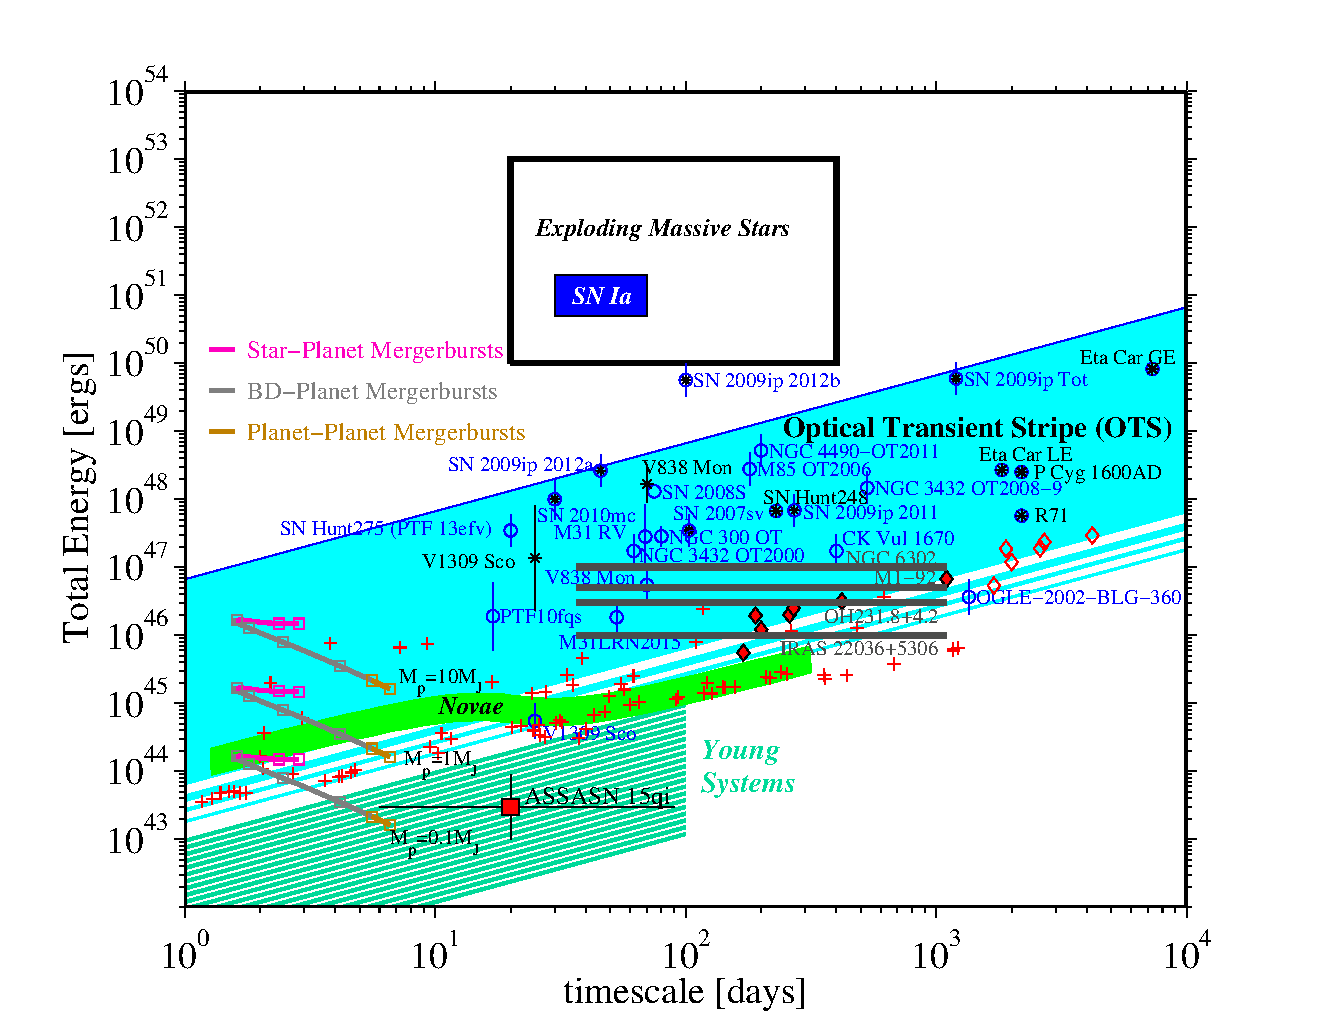
\includegraphics[width=1.0\textwidth]{etd.eps}
\end{center}
\caption{Energy-Time Diagram (ETD) of observed transient. The Optical Transient Stripe (OTS), is a more or less constant luminosity region in the ETD. It is populated by Intermediate Luminosity Optical Transients (ILOTs). The observed transients include a wide range of objects, probably powered by gravitational energy.
Some of the objects are merger events or vigorous mass transfer events (see \S\ref{subsec:Types of ILOTs}). Blue empty circles represent the total (radiated plus kinetic) energy of the observed transients as a function of the duration of their eruptions. The duration of an eruption is usually (but not always) defined as the time for the luminosity to decrease by 3 magnitudes $\Delta V=-3$. 
Mergerburst events are marked by blue filled circles.
The total energy does not include the energy which is deposited in lifting the envelope that does not escape from the star. Where a model exists to calculate the gravitational energy released by the accreted mass (the available energy) it is marked by a black asterisk.
The supernovae region is schematically marked by a rectangle. The green line represents nova models computed using luminosity and duration from \cite{1995ApJ...452..704D}. Nova models from \cite{2005ApJ...623..398Y} are marked with red crosses, and models from \cite{2010ApJ...725..831S} are represented with diamonds.
The four horizontal lines are not observed ILOTs, but rather represent the ILOT energy and duration as \cite{2012ApJ...746..100S} modeled for the formation of four bipolar planetary nebulae (PNe) and pre-PNe.
}\label{fig:ilot-club}
\end{figure}
%%%%%%%%

In the following, we discuss the common properties of ILOTs, and heir types.
Then, we focus on V838~Mon which will be at the focus of our research, and elaborate on the simulation we plan to perform and the goals we wish to achieve.

\subsection{Common Properties of ILOTs}
%------------------------

There are various models for different types of ILOTs (e.g., \citealt{2006A&A...451..223T,2007Natur.447..458K,2007Natur.449E...1P,2009ApJ...699.1850B,2009ApJ...697L..49S,2010ApJ...709L..11K,2010A&A...516A.108M,2010MNRAS.408..181P,2011A&A...528A.114T,2011MNRAS.415.2020S,2011MNRAS.415.2009S,2011MNRAS.415..773S,2011ApJ...730..134K,2014MNRAS.443.1319K,2015A&A...580A..34K,2016ApJ...817...66K,2018A&A...617A.129K,2019arXiv190100871J}).
As mentioned, \cite{2010ApJ...709L..11K} plotted the light curves in the optical band for different ILOTs with scaling of the time axis. 
It is evident that the \textit{decline patterns from the peak (or peaks) are similar, up to four magnitudes} (see Figure \ref{fig:0909.1909.TC1p2}).
They suggested that this implies that the same physical mechanism governs the different objects.
As mentioned above, \cite{2016RAA....16...99K} suggested that the source of energy in those similar ILOTs is gravity.
We will test this assumption using the simulations we propose to run.
%%%%%%%%
\begin{figure}[t!]
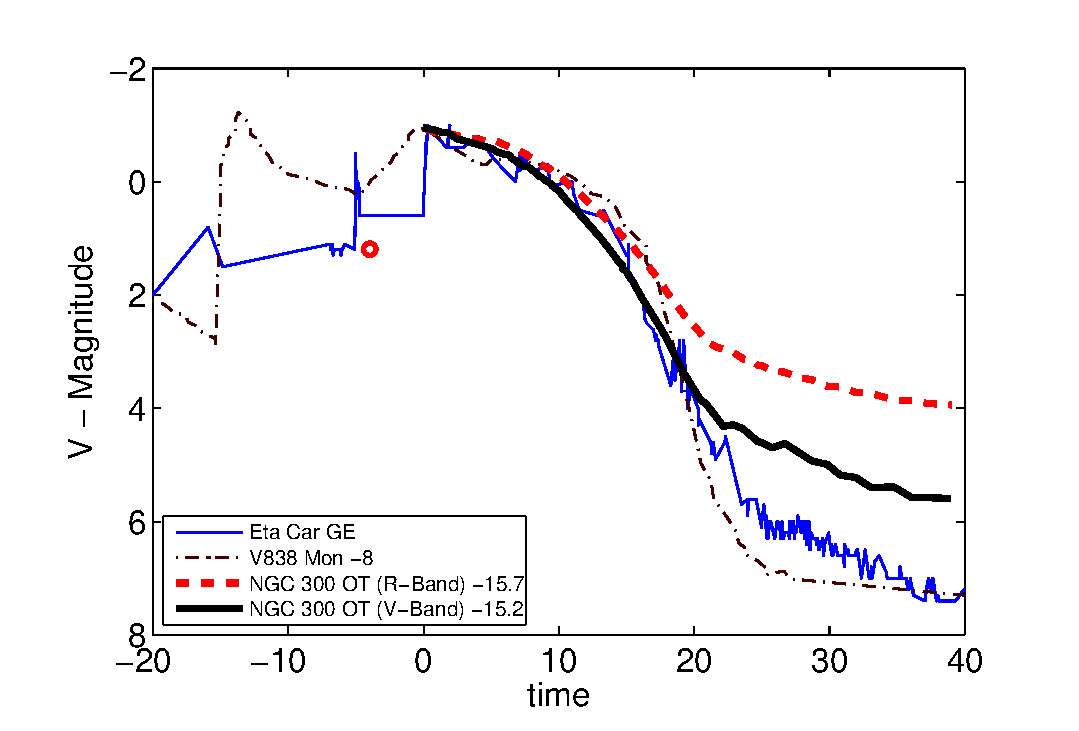
\includegraphics[width=\linewidth]{TC1p2.eps}
\caption{Comparison of the Visual band light curves of $\eta$~Car Great Eruption (GE), V838~Mon and NGC~300~OT. The timescale was normalized so that 1 time unit equals 1 year for $\eta$~Car GE, 2.2 days for V838~Mon, and 5.6 days for NGC~300~OT.
The curves translated vertically to bring peak luminosities to overlap (see legend for the shift values). 
It can be easily seen that the slope of the decline phase and its rate of change are similar for the three eruptions.
The same shape was later found to match the post-eruption light curves of other ILOTs.
We therefore think that there is a unique physical process that forms such a shape.
Figure adopted from \cite{2010ApJ...709L..11K}.}
\label{fig:0909.1909.TC1p2}
\end{figure}
%%%%%%%%%

To illustrate the merits of the merger and accretion models we discuss the High Accretion Powered ILOT (HAPI) model \citep{2016RAA....16...99K}.
We define $M_a$ and $R_a$ as the mass and radius, respectively, of star `a’ which accretes the mass. We will mark by `b’ the mass donor star.
We can estimate the average total gravitational power as
\begin{equation} 
L_G=\frac{ G M_a \dot M_a }{R_a}
\end{equation}
The angular momentum of the accreted mass implies the formation of an accretion disk, in case the specific angular momentum is high enough, or an accretion belt at the surface of the accretor if the specific angular momentum is low.
The viscosity time scale, which is the characteristic time for accretion from accretion disks, in the ILOTs we discuss here, is scaled according to
\begin{equation} 
T_{visc}\simeq \frac{R^2_a}{\nu} \simeq 73 \left(\frac{\alpha}{0.1}\right)^{-1} \left(\frac{H/R_a}{0.1}\right)^{-1} \left(\frac{C_s/\upsilon_\phi}{0.1}\right) ^{-1} \left(\frac{R_a}{5\Rsun}\right)^{3/2} \left(\frac{M_a}{8 \Msun}\right)^{-1/2} \text{days}
\end{equation}
Here $H$ is the hight of the disk, $C_s$ is the sound speed, $\alpha$ is the disk viscosity parameter, $\nu=\alpha C_s H$ is the viscosity of the disk, and $\upsilon_\phi$ is the Keplerian velocity, all taken in a representative radius in the disk. 
Using $M_a$ and $R_a$ scaled as in \cite{2005A&A...441.1099T}, according to the parameters of V838~Mon, viscosity to Keplerian timescale becomes $\chi \equiv t_{visc}/t_k\simeq 160$. 
We can write the accreted mass as $M_{acc}=\eta_a M_a$.
If we have a main sequence (MS) star that collides with a star (for example V838 Mon \cite{2006A&A...451..223T}) and tidally disrupts it the destructed star is likely to be less massive than the accretor $M_{acc} < M_b \lesim 0.3M_a$ and $\eta\lesim 0.1$.
The value of $\eta$ can differ quite significantly in different cases.
In a stellar collision, the star of the lower density will be the donor, namely, the one that is destroyed and accreted onto the other. But the star of the lower density does not have to be the less massive of the two.
For example, if both stars are MS star, the less massive of the two will be denser, and then  $\eta \gtrsim 1$). 
As another example if an evolved star loses a huge amount of mass but the accretor gains only a small fraction of the ejected mass (like in the great eruption of $\eta$~Car \cite{2008NewA...13..569K}), we will get $\eta\lesim 0.1$. 
These examples help us demonstrate why the range of $\eta$ can be large.
For simplicity, we will calibrate it to be $\eta \approx 0.1$, though values a dozen times larger or lower are also possible.
The viscosity time scale will be the minimum time scale for losing angular momentum and transferring material from the disk to the star (other processes such as radiative cooling may also be relevant, as well as possible instabilities in the disk). This gives an upper limit for the mass accretion rate
\begin{equation}
\dot M_a < \frac{\eta_a M_a}{t_{visc}} \simeq 4\left(\frac{\eta_a}{0.1}\right) \left(\frac{\alpha}{0.1}\right) \left(\frac{H/R_a}{0.1}\right) \left(\frac{C_s/\upsilon_\phi}{0.1}\right) \left(\frac{R_a}{5\Rsun}\right)^{-3/2} \left(\frac{M_a}{8\Msun}\right)^{3/2} \quad \msyr
\end{equation}
The maximum gravitational power is
\begin{equation}\label{eq.intro.LG}
L_G<L_{max} = \frac{GM_a\dot M_a}{R_a} \simeq 7.7 \times 10^{41}\left(\frac{\eta_a}{0.1}\right) \left(\frac{\chi}{160}\right)^{-1} \left(\frac{R_a}{5 \Rsun}\right)^{-5/2} \left( \frac{M_a}{8 \Msun}\right)^{5/2} \text{erg}~\rm{s^{-1}},
\end{equation}
where the parameters of the viscosity time scale are replaced with the ratio of the viscosity to the Keplerian time ($\chi$). 
The RHS of equation \ref{eq.intro.LG} fits such that it represents the top line of the OTS.
This luminosity is super-Eddington. 
For most ILOTs, the value of $\eta_a$ is such that they lay below the supper-Eddington line. 
Still, we see a large variability in $\eta_a$ and the accretion parameters. 
Also, we assume a thin accretion disk and the picture are much more complicated for a thick disk. 
A more accurate treatment requires hydrodynamic simulations together with radiation transfer. 
This proposal will focus on such solutions for some problems as is described later. 

\subsection{Types of ILOTs \label{subsec:Types of ILOTs}}
%------------------------
As we saw earlier the OTS in the ETD is quite wide, and includes objects that range from brown dwarfs (BD) to very massive stars (VMS).
\cite{2016RAA....16...99K} and \cite{2018Galax...6...82K} suggested classification in the following way, thoguh it is worth mentioning that there is still no consensus regarding the naming.

\begin{itemize}

\item \label{lrn-ilot-item} \emphbf{Luminous Red Nova (LRN) or Red Transients (RT) or Merger Bursts.} These designitions refer to quite diverse group describing transients powered by complete merger of two stars. 
The denser star tidally destroys the less dense star and accretes most of its mass. This releases gravitational energy that powers the event. Some mass from the destroyed star escapes the system.
This presents a characteristic merger light-curve. Examples for LRN include V838 Mon \citep{2005A&A...441.1099T}, V1309 Sco \citep{2011A&A...528A.114T}, and possibly eruptions of somewhat more massive progenitors, NGC~4490-OT \citep{2016MNRAS.458..950S} and M101~OT2015-1 \citep{2017ApJ...834..107B}.

\item \emphbf{Intermediate Luminosity Red Transients (ILRT).} 
The term refers to Asymptotic Giant Branch (AGB) stars or Red Giant Branch (RGB) stars that experience an ILOT event, most probable powered by gravitational energy of a companion that accretes mass from the giant star at a very high rate. Example include NGC 300 OT \citep{2009ApJ...695L.154B,2010ApJ...709L..11K,2016MNRAS.460.1645A}, SN 2008S and M31LRN 2015 \citep{2008ATel.1550....1P,2009ApJ...697L..49S,2009ApJ...705.1425P,2010MNRAS.403..474W,2016MNRAS.462..217S}.

\item \emphbf{Giant Eruptions (GEs).} These are eruptions of Luminous Blue Variables (LBVs) or other kinds of VMSs, designated also as atypical SN or SN impostors. GEs ILOTs typically characterize with the highest energy relative to other classes. The energy released in one or sequence of GEs can reach a few $\times10^{49} \erg$. Note that ILRTs are the low mass relatives of LBV GEs. Examples include the \nth{17} century GE of P~Cyg \citep{2010ApJ...723..602K,2018NewA...65...29M}, the \nth{19} century GEs of $\eta$~Car and the pre-explosion eruptions of SN 2009ip \citep{2016MNRAS.463.2904S}. 

\item \emphbf{ILOTs which created Planetary Nebulae (PNe).} There are noticiable similarities between some PNe and ILOTs \citep{2012ApJ...746..100S}: 
\begin{enumerate*}[label={(\alph*)}]
\item A short-duration event, which in some PNe is hinted upon from a linear velocity-distance relation in the nebula.
\item a bipolar structure;
\item a total kinetic energy of $\approx 10^{46}-10^{49}$ erg.
\end{enumerate*}
These similarities suggest that these PNe may have formed in an ILOT event lasting a few months. In the frame of the HAPI model the AGB or extreme AGB transfers mass on to a MS companion.
The velocity of the fastest gas parcels in such an outburst will be in the order of the escape speed of the MS star, namely a few $\times100 \kms$. 
Most of the gas is expected to interact with the AGB wind and slow down by a factor of 10 (i.e., to a velocity of ${\rm few} \times 10 \kms$).
\cite{2013MNRAS.436.1961A} conducted hydrodynamical simulations and demonstrated that a short jets-launching episode into an AGB wind, assumed to take place in a binary system, forms a bipolar PN with clumpy lobes. 
This might account, for example, to the bipolar PN NGC 6302, to the pre-PNe OH231.8+4.2 and M1-92, and to IRAS 22036+5306.

\end{itemize}

In addition to these ILOTs, more type of eruptions were suggested to populate regions in the continuation of the OTS and some of the less populated regions of the ETD. Among these we can count:

\begin{itemize} 
\item \emphbf{Weaker Mergerburst between a Planet and a BD.} According to this suggested scenario, a planet or a brown dwarf (BD) is shredded into a disk around a BD or a star respectively and the energy from accretion leads to an outburst \citep{2011MNRAS.416.1965B}. 
The process is a super-Eddington mergerburst that resides in the lower part of the OTS on the ETD.
In this process the plant destruction occurs before it plunges into the accreting object.
This is possible if the average density of the planet is smaller than the average density of the BD.
The planet must enter the tidal radius of the BD. 
For example, the orbit of the planet is perturbed to reduce the periastron distance, such that the planet gets into the tidal radius at periastron.
Once the planet is destructed as a result of the sequence of events, the remnant of the merger will resemble other LRNs but on shorter time scale and smaller energy.

\item \emphbf{A Weak Outburst of a Young Stellar Object (YSO).} YSOs may undergo unusual outbursts, such as the one observed in ASASSN-15qi \citep{2016ApJ...831..133H} or ASASSN-13db \citep{2017A&A...607A.127S}.
YSO outbursts are similar in many aspects to LRNe events like V838~Mon and V1309~Sco, but with lower total energy (and much fainter). 
Unlike LRNe that have a stellar secondary, the secondary object in YSO outbursts is smaller, in a size of a large planet.
The companion is tidally destroyed onto the primary YSO \citep{2017MNRAS.468.4938K}, releasing gravitational energy in the process.
These ILOTs differ from others, as they might reside \emph{below} the OTS even though the physical mechanism resembles LRNe.

\end{itemize}

ILOTs can also be classified according to the angle from were they are observed \citep[in a similar manner to the classification of galaxies and active galactic nuclii (AGN)][]{2015ARA&A..53..365N}:

\begin{itemize}
\item \emphbf{Type I ILOTs.} ILOTs which are deirectly observed. The condition for an ILOT to be classified as type I is that the observing direction is such that the ILOT is not obscured from the observer by an optically thick medium.
\item \emphbf{Type II ILOTs.}  Since most ILOTs are non-spherically symmetric eruptions we can expect that the same transient will appear differently only as a result of the point of view in the sky \citep{2017MNRAS.467.3299K}. 
This brings a new ILOT type, the Type II ILOTs.
The main property of this type is its orientation which makes the photosphere of the ILOT to be obscured.
Namely, the line of sight to the object intersects with a thick dust torus or an optically thick cloud.
A possible formation scenario for such an ILOT can be a strong tidal interaction at periastron passage in an eccentric orbit. 
The interaction leads to an axisymmetrical mass ejection which significantly departs from spherical symmetry.
This morphology is very common in progenitors of PNe (see \citealt{1987AJ.....94..671B,1995A&A...293..871C,1996iacm.book.....M,2011apn5.confP..21S,2016JPhCS.728c2008P}).
Such an eruption will be classified as type II if the light from the object is severely attenuated or hidden.
In most cases, the obscuring matter would reside in equatorial directions. 
The binary system will be obscured to the observer in the optical and IR bands as long as the dust has not dissipated.
A type II ILOT is accompanied by some polar mass ejection that may also form dust.
The dust in the polar directions interacts with the radiation that arrives from the central source.
We then can observe this reflected light which becomes much fainter and by doing so allowing the type II ILOT to be detectable. 
A possible example is the outburst of the red supergiant (RSG) N6949-BH1 in 2009 \citep{2017MNRAS.468.4968A}.

\end{itemize}


%----------------------
\section{The Model}
%----------------------

In the previous section we presented a wide range of supernova impostors and pointed out that a common process, liberation of gravitational energy, can presumably account for the observations.
As we discussed, the erupting sources have a large diversity.
In this section we seek to focus on one particular ILOT, and use it as a test case for many others.
Since the properties, and especially the light curves of many ILOTs are similar, generating the light curve based on a test-case would be a milestone in our understanding of these objects, and would justify our assumptions and our choice of a test-case object.
The test case we focus on is V838~Mon \citep{2005A&A...436.1009T,2006A&A...451..223T}, as a system of a product of stellar merger event (``mergerburst''), consists of a massive accretion disk around a star.

\subsection{ILOT model and V838~Mon}
LRN come with a large range of initial masses, e.g., V838~Mon is $\sim5-10 \Msun$ \citep{2006A&A...451..223T}, M101~OT2015-1 ia about $\sim18 \Msun$   \citep{2017ApJ...834..107B} and NGC~4490-OT is around $\sim30 \Msun$ \citep{2016MNRAS.458..950S}.
According to the V838~Mon model, we have a process in which energy of $2.5 \times 10^{46}~\erg$ is released on a time scale of about one month.
The most probable process for emitting a large amount of energy for an extended duration of time is accretion through a disk.
Accretion onto a MS star with luminosity of $\sim 10^6 ~ \Lsun$ requires an accretion rate of $\sim 0.01 \msyr$.
In V838~Mon we need to accrete $\geq 0.1 \Msun$ on a time scale of months.
During the main outburst of V838~Mon (January -- mid April 2002) the system lost $\sim2.5\times10^{46}$ erg in radiation and approximately $0.01-0.1 \Msun$ in mass (observed by lines) with velocities of $\approx 300 \kms$.
The energy necessary to lift this amount of material from the surface of a star having $M_{\star}=8 \Msun$ with $R_{\star}=5 \Rsun$ and to accelerate it to $300 \kms$ at large distances is $(0.4-4)\times 10^{47} \erg$.
Binary system with a stellar donor, even a close binary with Roche Lobe Overflow, cannot account for the desired light curve as there is no mechanism to accrete on a very short time such a large amount of mass.
The most promising model to account for V838~Mon $2002$ outbursts is a main sequence and pre-MS companion merger with a highly eccentric orbit inflating huge envelope with mass loss and wind \citep[see][and within]{2006A&A...451..223T,2007ASPC..363..280S}.
In later phases the evolution of a merger remnant will be governed by the gravitational contraction of its inflated envelope.

The mass loss rate can vary with time. In the eruption of V838~Mon three peaks were observed, which were associated with three eruptions.
We expect to have the a similar imprint in the mass loss in our simulation, perhaps as a result of instabilities in the disk.
The (abrupt) variation in the mass loss rate will effect the velocity and density fields
\begin{equation}
    \rho(r,t)=\frac{\dot{M(t)}}{4 \pi r(t)^2 v(r,t)},
\end{equation}
and as we will measure the variation we will be able to deduce the corresponding change in the location of the photosphere $R_{ph}(t)$ according to
\begin{equation}
    \int_{\infty}^{R_{ph}} \kappa(r,t) \rho(r,t) \,dr = \frac{2}{3}.
\end{equation}
With this calculation we can numerically find $R_{ph}(t)$ and make a comparison to the photospheric radius derived by \cite{2005A&A...436.1009T} for V838~Mon.

We seek to achieve a numerical model that can reproduce some of the typical observation of V838~Mon.
\begin{enumerate*}[label={(\alph*)}]
\item Luminosity of $\sim 10^6 \Lsun$ \citep{2005A&A...436.1009T};
\item Aspherical envelope (thick disk) \citep{2005ApJ...622L.137L};
\item Mass loss of about $0.3 \Msun$ (for constant gray opacity using Rosseland mean opacity). \citep{2007ASPC..363..161H,2007ASPC..363...13M};
\item Envelope radius $\sim 500$-−$1500R_\odot$ \citep{2007ASPC..363..280S};
\item Temperature of $T_{eff} \approx 4\times10^3\K$ \citep{2005A&A...436.1009T,2007ASPC..363..225P};
\item Wind Velocity of about $\sim 300 \kms$ \citep{2006A&A...451..223T,2007ASPC..363...13M};
\item Energy of $(0.4{-}4.0) \times 10^{47} \erg $ \citep{2005A&A...436.1009T};
\item Photospheric radius as a function of time \citep{2005A&A...436.1009T}.
\end{enumerate*}



We point out, as \cite{2006A&A...451..223T} (section \S4.2) state, that the main drawback of the merger model is that it is based
on estimates and approximate considerations \citep[see also][]{2007ASPC..363..280S}
and should be carefully tested and validated with detailed numerical simulations.
Our Simulations will overcome this drawback, by following a detailed scenario, with a code that has all the relevant physics incorporated inside, allowing to validate the assumptions and obtain meaningful results.


\subsection{Guidelines for the proposed simulation}

In a merger process the lower-density object is destructed onto the higher density one. We assume that eventually the destructed star forms a thick disk around the other star. 
Another proposed scenario for merger is a binary system with common-envelope evolution (CEE) during which two stars orbit inside a single, shared envelope \citep[see][and within]{2013A&ARv..21...59I}.
%Here, a higher density object dives into the envelope of the companion, for example, a main sequence star enters into a red giant star envelope \citep[for more details on CEE see][and within]{2013A&ARv..21...59I}.

In addition to the model of \cite{2005A&A...436.1009T} and \cite{2006A&A...451..223T} and its following development, we wish to add a a full investigation of the shape of the lightcurve.
We focus on the lightcurve after the series of peaks (that is probably the result of a spiraling companion being destructed), when the accretion is continuous and the luminosity declines.
As the shape of the light curve is not unique for V838~Mon, but rather common to many ILOTs (see section \S \ref{lrn-ilot-item}), we think that obtaining the shape of the lightcurve is important to the physical understanding of ILOTs in general and V838~Mon in particular.
The observed light curve is a consequence of the following process:
\begin{enumerate}
    \item Accreting from a disk or a thick belt and obtaining the rate of gravitational energy released during the process. For that purpose the physical properties of the star$+$disk system need to be mimicked \citep{2005A&A...434.1107M,2005A&A...441.1099T,2006CBET..780....1M,2007ASPC..363.....C} in the best possible way.
    \item The way the energy travels through the ambient medium and interacts with the gas, by absorption and scattering.
    \item The line-of-sight to the object, that will determine whether the ILOT is observed directly or indirectly by reflection (according to the line of sight we classify the ILOT as type~I or type~II).
    \item The amount of light gathered in the observed bands according to the response of each of the telescope filters.
\end{enumerate}

We propose to simulate a post-stellar merger scenario that can result in the required light-curve. Namely, we intend to start with a star$+$disk system, which is assumed to be the product of the merger process.

\subsection{Simulation tools}
We will use version 4.5 of the \flash{}\footnote{\url{http://flash.uchicago.edu}} hydrodynamic code \citep{2000ApJS..131..273F}. It is a well-tested publicly available multiphysics multiscale simulation code with a wide international user base routinely used by many astrophysicists. It has a wealth of documentation, help resources and complementary tools. It is an Eulerian hydrodynamics code with adaptive mesh refinement (AMR) including robust solvers for hydrodynamic like the well-known piecewise-parabolic method \citep[PPM; ][]{1984JCoPh..54..174C}. Alongside \flash{} we will use \radmc\footnote{\url{http://www.ita.uni-heidelberg.de/ dullemond/software/radmc-3d/}} \citep{2012ascl.soft02015D} a freely available and open source Monte Carlo radiative transfer code used in astronomy.% and astrophysics. 
It calculates, for a given geometrical distribution of gas and dust, what its spectra look like when viewed from a certain angle. The code is well documented and has numerous simple examples that can be used as templates. To orchestrate the two, and for visualizating the simulation, we will use \yt{}\footnote{\url{https://yt-project.org/}} \citep{2011ApJS..192....9T} integrated science environment.

\subsection{Setup}
\label{sec:setup}
We setup initial conditions of a star that just completed a merger burst event.
The thick disk originated from the destruction of the companion.
The disk mass will be $0.1$--$1 \Msun$ and it will be covering a semi-angle of $30 \deg$ around the equator for a radius of about $R\sim10$--$15 \Rsun$ forming a shape that resembles a torus (hereafter `the torus', or `the disk').
The mass of the primary star that was not destructed in the merger burst is $8 \Msun$ and its radius is $5 \Rsun$.
We use for the initial conditions a gas dominated spinning tours in a Keplerian velocity follow the thick disk model given in \cite{2002apa..book.....F} Ch.10 and Ch.11 (see \S\ref{app:thick_disk_model}). Namely, the radiation pressure is assumed to be small compared to the gas pressure.


We expect a massive outflow from the disk in the form of jets or wide bipolar disk wind \citep[see][]{2018ApJ...868..136M,2019arXiv190203931S}.
In order to study the effects one-by-one, adding the jet will be done separately, in a later stage.
The formation of jets have yet to be derived by simulations
We will therefore manually insert an outflow to the simulation as needed.



We do not know what the temperature of the disk would be after the complicated process of destruction, so we will test a number of values for the initial disk temperature, in the range of $10^4$--$10^6 \K$.
The disk composition is taken from the companion star to be of solar composition $X=0.7$ and $Y=0.28$.
The following initial disk dimensionless parameters holds and give better understanding of the fluid flow: 
\begin{enumerate*}[label={(\alph*)}]
\item Toomre’s parameter \citep{1964ApJ...139.1217T} $Q=c_s\kappa/\pi G \Sigma > 1$, and thus the disk is stable against gravitational fragmentation;
\item Reynolds numbers $R_e=\rho u l / \mu>>1$;
\item Knudsen number $K_n=\lambda_\gamma / R < 1$, where $\lambda_\gamma$ is the gas mean free path.  We can use continuum mechanics to describe the problem;
\item Magnetic Reynolds number $R_{en}= c_s H/ \eta <<1$, where $\eta$ is the magnetic diffusivity of the fluid We can therefore neglect the Magneto-Hydro-Dynamic (MHD) effects.
\end{enumerate*}

We expect the disk to undergo instabilities \citep{1988MNRAS.232....1F,2018ASSL..454.....S}
such that part of the energy in the disk will be dissipated and part of the gas in the disk will be accreted onto the primary star.
We will be able to quantify the accretion rate and identify the directions from where the accreted material arrives onto the star similar to \cite{2018arXiv180502529K,2018Galax...6...82K}.

We will take frequent snapshot from the \flash{} simulation and postprocess them in \radmc{}.
This will allow us to derive Spectral Energy Distribution (SED), and determine the luminosity as a function of time in each waveband (in optical and near-IR) as seen by an observer.
We will test different lines of sight, as the same eruption can look very different from different lines of sight \cite{2017MNRAS.467.3299K}.
This will allow us to compare the simulate transient light curve to the observed one.
We will test many parameters to cover as much as possible of the parameters space. E.g, different masses in the disk, covering fraction of the disk (angle), artificial viscosity values, etc.

\section{Road-Map}

In order to reach our goals, we presents the project main checkpoints:
\begin{enumerate}
\item Setting-up a Linux developer machine running \flash{}, \radmc{}, \visit{}, \yt{} and all the companion software development environments like openMPI, HDF5, IDEs, etc.
\item Running \flash{} hydrodynamic 3D test code on coarse grid. Running the Keplerian rotating torus test case. We will use \visit{} for inspecting the results.
\item Adding codes that treat more physical processes into the test case, such as multi-species (composition), multi-gamma equation of state and radiation transfer.
\item Integrating \radmc{} code for post-processing the \flash{} simulations.
\item Adding post processing visualization routines using \yt{}.
\item Managing the simulations using \python{}. Running \flash{} and \hbox{\radmc{}} automatically from \python. Running some hydrodynamic steps then do \radmc{} post-processing and if necessary continuing with the simulations iteratively to get a wide observation like picture.
\item Debugging and collective test the code (reliability) on coarse grid.
\item Exporting the code to a high power computer (HPC). Running the thick disk accretion model on a fine grid.
\item Full scale running (production simulations).
\item Analyzing the results and summarizing them.
\item Exploring the parameter space.
\end{enumerate}


\section{Preliminary result\label{app:preliminarty result}}
We present the initial result of the simulation discussed in section \S\ref{sec:setup}. This section demonstrates that we have the required expertise and numerical tools to setup and run the proposed simulation. We present a \flash{} setup with central star of $8\Msun$ in the center surround with thick accretion disk, a torus like, of $1 \Msun$ with Keplerian velocities. We show here only the first step into the simulation at low resolution, and the production simulations will be of much higher quality.

In Figure \ref{fig:preliminary-result-density} we show the border lines of the density as a iso-surface color with red and the Keplerian velocity between the upper and lower surface showing the disk matter movement. The green circular glyphs represent the Keplerian velocity of the thick disk. The density distribution in the disk is small and we discard their iso-surface for clarity. In the upper view we see a blue glyphs represent the ISM, a very low density region of $\approx 10^{-10} \g\cm^{-3}$, attract to the central object.
The ISM is initialized with zero velocity and quickly falls into the central object. Figure \ref{fig:preliminary-result-velocity} shows the same snapshot of the simulation focus on the velocity field.  
The gravitational field is due to that star as a central object (as a point mass), as the mass in the disk is significant, we will switch to self-gravity solution.

%
\begin{figure}[t!]
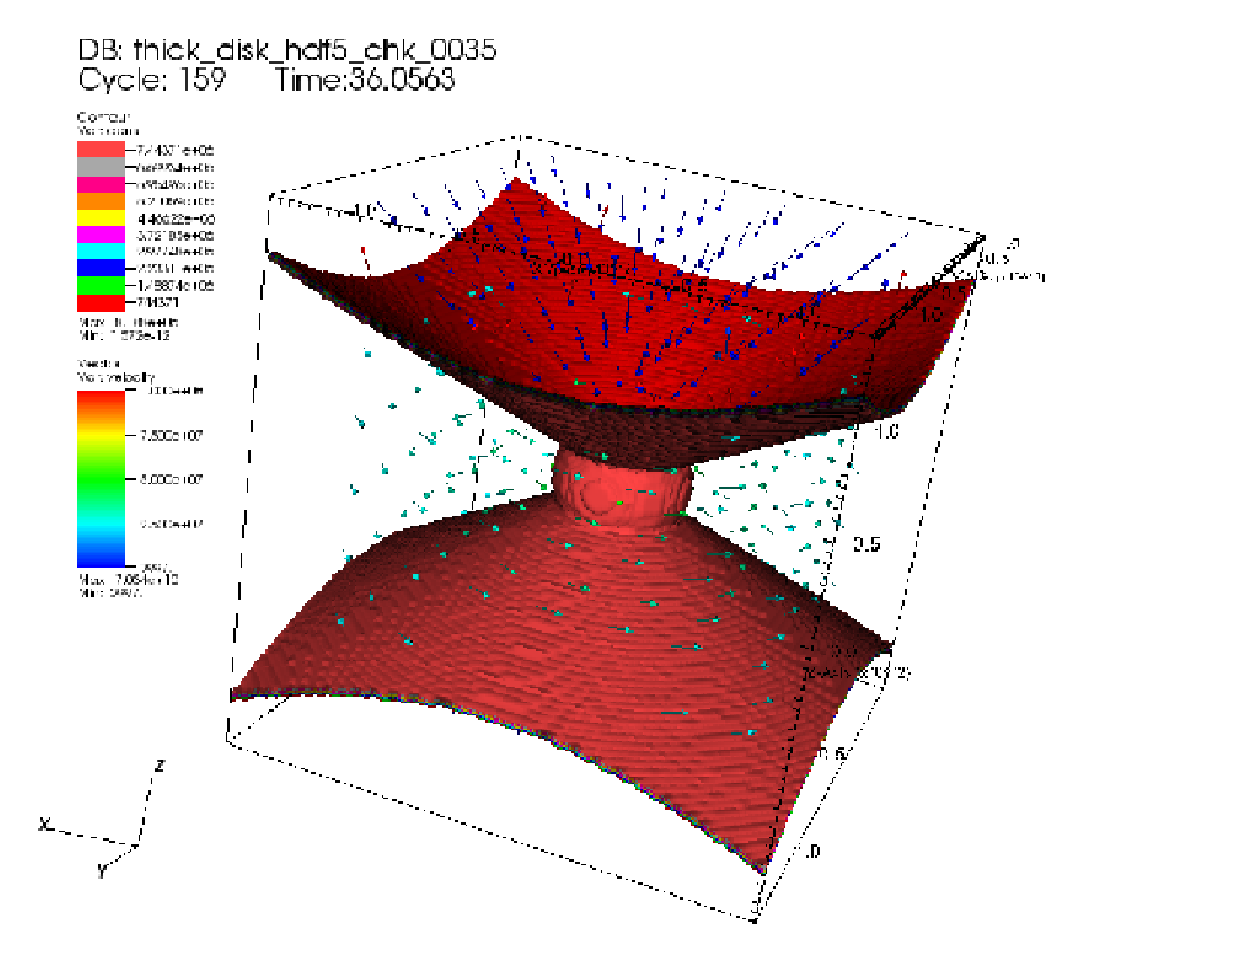
\includegraphics[width=\linewidth]{visit_dens_1.eps}
\caption{The simulation snapshot after a few steps showing the system setup. The iso-surface of the density color with red. The volume between the surfaces are filled with matter and the variation in the density is very small so we discard the relevant iso-surfaces for clarity. The matter between the surfaces form the thick disk and it initially set to Keplerian velocity distribution. The matter outside the surfaces are filled with ISM like matter with no velocity.}\label{fig:preliminary-result-density}
\end{figure}
%
\begin{figure}[t!]
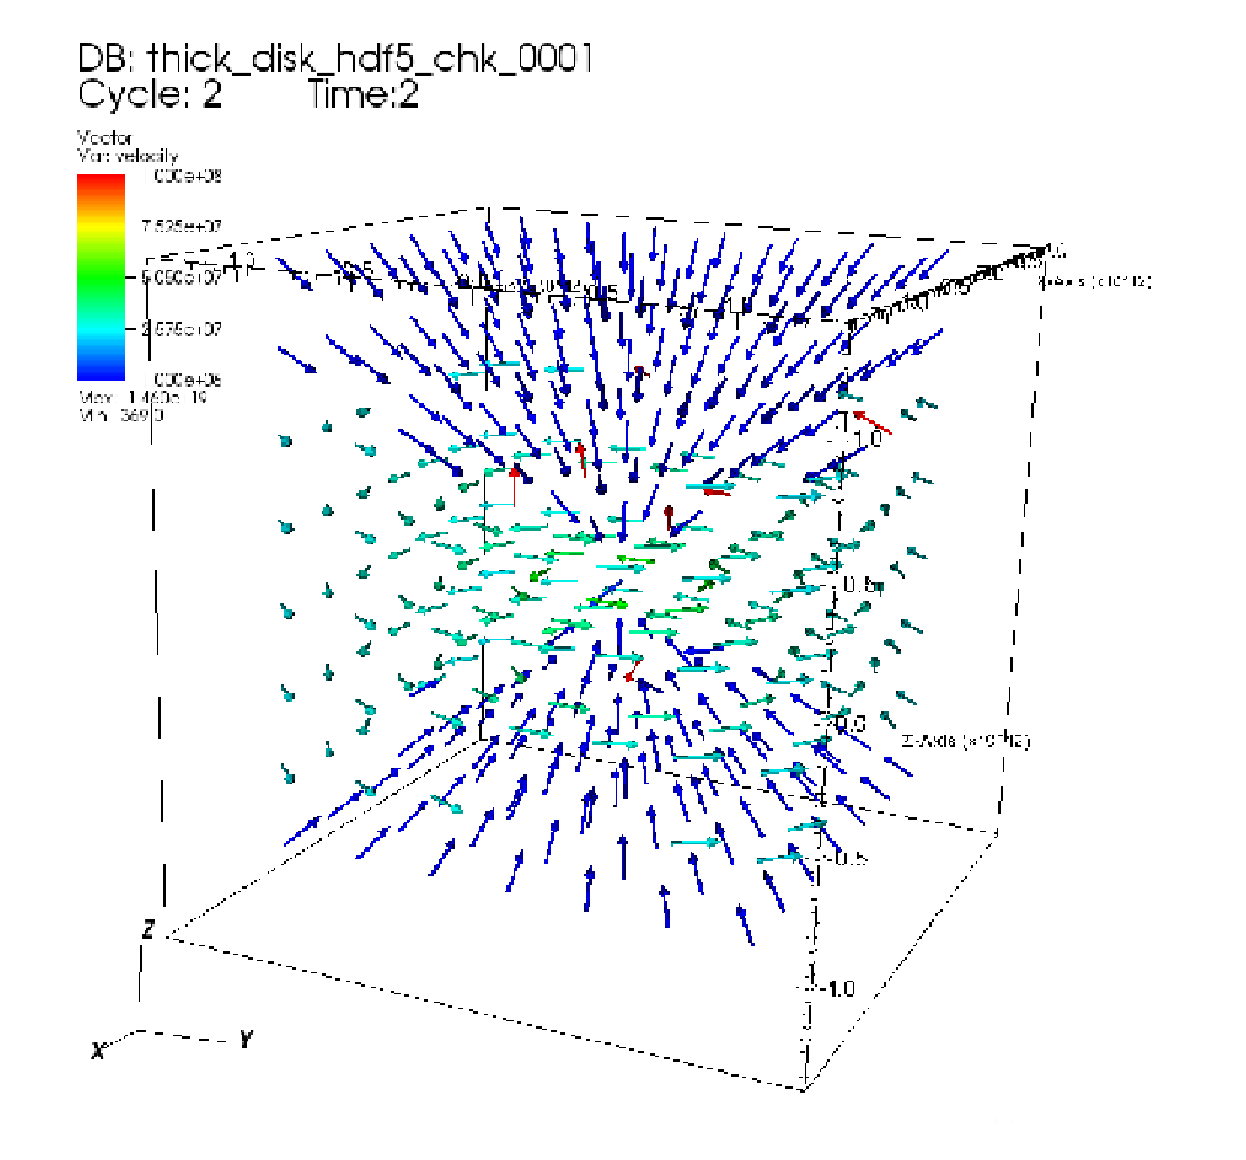
\includegraphics[width=\linewidth]{visit_vel_1.eps}
\caption{The velocity field, a few time steps after the onset of the simulation. The green glyphs are the thick disk Keplerian distribution and the blue glyphs represent the ISM matter fall into the central object as it start with zero velocity.
In our simulations we will switch from point-mass gravity to self gravity. We will also add manually launched jets, in a later stage.
}\label{fig:preliminary-result-velocity}
\end{figure}

%\vspace{1cm}
\section*{Acknowledgement}
We thank Prof. Noam Soker for the Technion, who is an expert on the topic of the research proposal for very helpful comments that helped improving it.
\appendix


%\section{Polytropic Envelope\label{app:polytropic_envelope}}
%TBA

\section{Thick Disk Model\label{app:thick_disk_model}}
In this appendix we present the thick disk model as discussed in the literature. The case of thick disk is still under development and rises theoretical and observational questions. There is a large number of works indicating that thick disks play an important role in AGN. There also indication that thick disks rise in stellar mergers, generation of bipolar outflows and jets and early stages of star formation.
As a result, there is no consensus for a `textbook' thick disk solution. Instead, there is a widely used guideline of the torus model.
We will follow \cite{2002apa..book.....F} book, but first let us present a few hydrodynamic governing equations.

We start with conservation of mass (continuity equation),
\begin{equation}\label{eq:conservation_of_mass}
\frac{\partial \rho}{\partial t} + \frac{\partial (\rho u_k)}{\partial x_k} = 0
\end{equation}
Where $\rho$ is the matter density and $u_k$ is the fluid velocity.
We continue on to conservation of momentum,
\begin{equation}\label{eq:conservation_of_momentum}
\rho\frac{\partial u_j}{\partial t} + \rho u_k \frac{\partial u_j}{\partial x_k}=\frac{\partial \sigma_{ij}}{\partial x_i}+\rho f_j
\end{equation}
Where $f_i$ is body forces per mass, $\sigma_{ij}$ defined as, 
\begin{equation}
\sigma_{ij} \equiv -p\delta_{ij}+\tau_{ij}
\end{equation}
p is the pressure and $\tau$ is the shear stress tensor
\begin{equation}
     \tau_{ij} = \lambda \delta_{ij} \frac{\partial u_k}{\partial x_k}+ \mu \left( \frac{\partial u_i}{\partial x_j} + \frac{\partial u_j}{\partial x_i} \right)
\end{equation}
$\lambda$ and $\mu$ are the dynamic viscosity and second viscosity coefficient. Usually the kinematic viscosity defined as $\nu = \mu/\rho$. The second viscosity coefficient can be represent as $\lambda = \K - 2\mu/3$, $\K$ is the bulk viscosity defined as
\begin{equation}
    p-\bar p = \K \frac{\partial u_k}{\partial x_k} 
\end{equation}
which for incompressible fluid leads to Stokes relation $\lambda = - 2\mu/3$.
The conservation of energy equation is,
\begin{equation} \label{eq:conservation_of_energy}
\rho\frac{\partial e}{\partial t}+\rho u_k \frac{\partial e}{\partial x_k} = \sigma_{ij} \frac{\partial u_j}{\partial x_i} - \frac{\partial q_j}{\partial x_j}, 
\end{equation}
where $e$ is the intrinsic energy of the fluid per mass, 
\begin{equation}
q_j \equiv -\kappa \frac {\partial T}{\partial x_j}    
\end{equation}
is the heat flux leaving the fluid, and $\kappa$ is the thermal conductivity.

The set of equations \ref{eq:conservation_of_mass}, \ref{eq:conservation_of_momentum} and \ref{eq:conservation_of_energy} with two equations of state, for the pressure $p=p(\rho,T)$ and for the internal energy $e=e(\rho,T)$, constitutes the Navier-Stokes equations. 
The disk equation (and \flash{}) derived from this set of equations with different physics lead to different terms and approximations (different representation of the equations. 
For a more detailed discussion on fluid flow see \citealt{currie2002fundamental}).

%Equipped with Navier-Stokes we move to toroidal equilibria without accretion solution (\cite{2002apa..book.....F} Ch.10) as a representation of thick disk.
Thick disk may form during the merger of two stars as the system attempts to handle its excess angular momentum.
As we shall see, these thick disk may possess a narrow funnel along the rotation axis where large radiative pressure gradients can accelerate matter in collimated jets. 
The thick disk solution is a feasible model for a transient which derives its power from accretion and intrinsically generates jets without any extra assumptions (e.g. magnetic fields, a confining cloud, etc).

We will now describe the structure and shape of pure (with no viscosity) rotating fluid in about its axis of symmetry in cylindrical system of coordinates $(R,\phi,z)$. 
The velocity field has the components: 
\begin{equation}\label{eq:velocity_field_components}
V_R=0, \quad v_\phi=R\Omega, \quad v_z=0,
\end{equation}
where $\Omega$ is the angular velocity (e.g., for thick Keplerian disk $\Omega=\sqrt{G M_\star / R^3}$).
Navier-Stokes equations for inviscid fluid in cylindrical coordinates reduce to
\begin{equation}
% equations of motion of an inviscid fluid subject to gravitational forces (including external bodies)
\begin{split}
\label{eq:inviscid_fluid}
\frac{1}{\rho} \frac{\partial P}{\partial R} &= - \frac{\partial \Phi}{\partial R} + \Omega^2R,  \\
\frac{1}{\rho} \frac{\partial P}{\partial z} &= - \frac{\partial \Phi}{\partial z} ,
\end{split}
\end{equation}
where $P$ is the pressure and $\Phi$ is the gravitational potential.
Notice that the equations in vector form are:
\begin{equation}\label{eq:vector_inviscid_fluid}
\frac{1}{\rho}\mathbf{\nabla} P = -\mathbf{\nabla}\Phi+\Omega^2\mathbf{R} = \vec{g_{\rm{eff}}}
\end{equation}
We defined the effective gravity $\vec{g_{\rm{\rm{eff}}}}$ as the vectorial sum of gravitational and centrifugal acceleration. Therefore the isobaric surface is perpendicular to $\vec{g_{\rm{eff}}}$ at any point.
So we can write along the isobaric surface (denoted by subscript s):
\begin{equation}
\frac{\partial g_{\rm{eff}}}{\partial R} dR_s + \frac{\partial g_{\rm{eff}}}{\partial z} dz_s =0
\end{equation}
Using \ref{eq:inviscid_fluid} along the definition of effective gravity we get:
\begin{equation}\label{eq:surface_differential}
\left( \Omega^2R \right)_s = \left( \frac{\partial \Phi}{\partial z} \right)_s \frac{\partial z_s}{\partial R_s} + \left( \frac{\partial \Phi}{\partial R} \right)_s
\end{equation}
Now suppose a cloud of negligible mass rotates around a point mass $M_\star$ with angular velocity $\Omega$ such that 
\begin{equation}
\Omega^2=\frac{GM_\star e^2}{r^3}=\frac{GM_\star e^2}{(R^2+z^2)^{3/2}}
\end{equation}
With $\Phi=-GM_\star/r$.
We can integrate directly equation \ref{eq:surface_differential} to yield the meridional cross-section of our disk
\begin{equation}
(1-e^2)R^2+z^2=\rm{constant}=z^2_P
\end{equation}
This result indicates $P=P(z_P)$ and from equation \ref{eq:inviscid_fluid} we can solve for the density:
\begin{equation}
\frac{1}{\rho}=-\frac{\partial \Phi}{\partial z} / \frac{\partial P}{\partial z}
\end{equation}
Which leads to 
\begin{equation}
\frac{\partial P}{\partial z} = \frac{\partial P}{\partial z_P}\frac{\partial z_P}{\partial z} = \frac{\partial P}{\partial z_P}\frac{z }{z_P}
\end{equation}
Thus we can obtain the solution for the density
\begin{equation}
\frac{1}{\rho}=-\frac{GM_\star z_P}{r^3(dP/dz_P)}
\end{equation}
From this result we see that a physically plausible equilibrum requires $dP/dz_P<0$, namely pressure must decrease outwards in order to balance gravity. 
Activating the curl operator ($\mathbf{\nabla}\times$) on both sides of equation \ref{eq:vector_inviscid_fluid} and using  \ref{eq:velocity_field_components} we get
\begin{equation}
    \vec\nabla\left(\frac{1}{\rho}\right)\times\vec\nabla P = 2\Omega \vec\nabla \Omega \times \vec R = 2\frac{\partial \Omega}{\partial z} \vec v
\end{equation}

The vectors $ \vec\nabla\left(\frac{1}{\rho}\right)$ and $\vec\nabla P$ are orthogonal to isopycnic (constant density surface) and isobaric surfaces respectively.
If $\partial \Omega/ \partial z=0$ everywhere, the result with the two vectors must be parallel everywhere, the surfaces of constant pressure and constant density are coinciding, and this also implies that $\Omega=\Omega(R)$ for non-vanishing rotation. This result simplifies considerably the task of finding the structure of the disk when the angular velocity is constant on cylinders. Also another immediate result is that the pressure and density must be functionally related $P=P(\rho)$.
As result of $\partial \Omega/ \partial z=0$ it is possible to introduce a rotational potential $\psi_{\rm{rot}}$ such that
\begin{equation}
\Omega^2(R)\vec R = \vec \nabla \psi_{\rm{rot}}
\end{equation}
Where 
\begin{equation}
\psi_{\rm{rot}} = \int^R  \Omega^2(R') R' d R'
\end{equation}
Then form equation \ref{eq:vector_inviscid_fluid} we have $\Phi_{\rm{eff}}=\Phi-\psi_{\rm{rot}}$ and $\vec g_{\rm{eff}} = -\vec \nabla \psi_{\rm{eff}}$ so that the equation for isobaric/isopycnic surface becomes simply 
\begin{equation}\label{eq:phi_eff_constant}
\Phi_{\rm{eff}}=\Phi-\psi_{\rm{rot}}=\rm{constant}
\end{equation}
In this configuration the surfaces of constant pressure, density and effective potential all coincide. Therefore finding the shape and stratification of the disk is reduced to obtaining the equipotentials of $\Phi_{\rm{eff}}$. As we know a priori the gravitational potential this task is relatively simple. So we may use $\Phi_{\rm{eff}}=\Phi(R,z)-\psi_{\rm{rot}}(R)=\rm{constant}$ to obtain the equlibrium rotation field for a given equipotential shape result with
\begin{equation}\label{eq:rotation_potantial}
    \psi_{\rm{rot}}=\Phi(R,z_s(R))
\end{equation}
where $z=z_s(R)$ is the equation for the cross-section of the surface.

Now consider a disk surface generated by revolution of two straight lines at angles $\pm\alpha$ to the equatorial plane. Let us assume the disk self gravity is negligible and that it is in equilibrium with the gravitational field of point mass $M_\star$ at the origin.
The equation for the cross-section of the disk angular half-thickness angle $\alpha$ is
\begin{equation}
z_s(R)=\pm(\tan\alpha)R
\end{equation}
As all the conditions required for the validity of \ref{eq:rotation_potantial} are met, we substitute this into the potential of the point mass to obtain
\begin{equation}
    \psi_{\rm{rot}}(R)=\frac{GM_\star \cos \alpha}{R}
\end{equation}
and for angular velocity 
\begin{equation}\label{eq:angular_velocity}
    \omega^2=\frac{1}{R}\frac{\partial \psi_{\rm{rot}}}{\partial R} = \frac{GM_\star\cos\alpha}{R^3}
\end{equation}
The equilibrium rotation field is `Keplerian' but corresponds to a mass $M_\star\cos\alpha<M_\star$, where the velocities are less then Keplerian velocities because the pressure distribution necessary to support the disk vertically has a radial gradient. From \ref{eq:phi_eff_constant} where we set $\Phi_{\rm{eff}}\neq0$ we get one parameter family $\Phi_{\rm{eff}}$ for the internal pressure and density stratification layers
\begin{equation}
    r= - \frac{GM_\star}{\Phi_{\rm{eff}}}
    \left(1- \frac{\cos\alpha}{\cos\lambda} \right)
\end{equation}
where $\lambda$ is the latitude. 
For small values of $\alpha$ we notice that $|\partial P/\partial z| \gg |\partial P/\partial R|$. This result also characterize a range of thin accretion disk.
\begin{figure}[ht!]
\includegraphics[width=\linewidth]{meridional_equipotentials_section_z–R_plane_thick_disk.png}
\caption{Meridional equipotentials section in the z–R plane, surface given
by $z_s=\pm(\tan \alpha)R$. The bound fluid $E < 0$ is shown shaded.}
\label{fig:thick-disk-tori-struct}
\end{figure}

After gaining some insights into the thick disk geometric structure, we look into some details about the disk luminosity. We show that the disk can exceed the Eddington limit by a large factor. If the disk contains a hollow axial region (this is true for a large class of thick disk objects), commonly known as the `funnel’, in this region the centrifugal force always exceeds gravity such that the balance between the pressure gradients and rotation determines the disk equilibrium.
As it turns out the maximum radiative output in this thick disk funnels objects related to rotation rather than to the central mass and therefore can exceed $L_{\rm{Edd}}$.
Before we begin let us make some order of magnitude estimation. 
For nuclear processes ($\rm{H}\rightarrow \rm{He}$) we can get about $\sim 0.007~mc^2$ in energy, for accretion we can have $\sim R_{\rm{Sch}}/(2R) ~ mc^2$ where for example $R<70R_{\rm{Sch}}$ we get $\sim 1/(2\cdot 70) ~mc^2 \sim 0.05~mc^2$. That accretion process can easily be more efficient. 
The radiation force can roughly be estimated as 
\begin{equation}
F_{out}=\frac{\sigma_T L_\star}{4\pi r^2 c}
\end{equation}
Where we use Thomson scattering (ionized hydrogen of free electrons) cross section $\sigma_T=6.65 \times 10^{-25} \cm^2$.
The inward balancing gravitational force on the electron proton pair is 
\begin{equation}
F_{in}=\frac{GM_\star m_p}{r^2}.
\end{equation}
Comparing the two result with Eddington luminosity 
\begin{equation}
L_{\rm{Edd}} = \frac{4\pi G M_\star m_p c}{\sigma_T}\simeq 3.4\times 10^4  \left( \frac{M_\star}{\Msun} \right) \Lsun
\end{equation}
If the entire gravitational energy emitted as radiation 
\begin{equation}
L_{acc} = \frac{G M_\star \dot M}{R_\star} =
5.02 \times 10^7  \left(\frac{M_\star}{8 \Msun}\right) 
\left(\frac{\dot M}{1 \msyr}\right) 
\left(\frac{R_\star}{5 \Rsun}\right)^{-1} \Lsun
\end{equation}
And taking in to account the Eddington limit we get
%\begin{equation}
%\begin{split}
%\dot M_{\rm{Edd}} = \frac{4\pi m_p c R_\star}{\sigma_T} \\
% %\dot M_{\rm{Edd}} \approx 9\cdot10^{16} gram~sec^{-1} %\left(\frac{R_\star}{1 ~km}\right) \\
%\dot M_{\rm{Edd}} \approx 1\cdot10^{-1} M_\odot ~Yr^{-1} \left( %\frac{R_\star}{R_\odot} \right)
%\end{split}
%\end{equation}
\begin{equation}
\dot M_{\rm{Edd}} = \frac{4\pi m_p c R_\star}{\sigma_T} ,
\end{equation}
that can be calibrated as
\begin{equation}
\dot M_{\rm{Edd}} \simeq 0.1  \left( \frac{R_\star}{\Rsun} \right) \msyr.
\end{equation}
We can define the disk black-body temperature as
\begin{equation}
\begin{split}
T_b &=\left(\frac{L_{acc}}{4 \pi R_\star^2 \sigma} \right)^{1/4} \\
 &= 21.73 \times 10^4 
\left(\frac{M_\star}{8 \Msun}\right)^{1/4}
\left(\frac{\dot M}{1 \msyr}\right)^{1/4}
\left(\frac{R_\star}{5 \Rsun}\right)^{-3/4} \K \\
\end{split}
\end{equation}
and the disk thermal temperature as ($3kT_{th}\simeq GM_\star m_p / k R_\star$)
\begin{equation}
T_{th}= \frac{GM_\star m_p}{3 k R_\star}.
\end{equation}
In general we have
\begin{equation}
T_b \leq T_{rad} \leq T_{th}
\end{equation}
for radiation from an optically thick disk that is in equilibrium with the thermal temperature $T_{rad}\sim T_{th} \sim T_b$ .

The radiative flux in equilibrium can be write as
\begin{equation}
\mathbf{F}= -\frac{C}{\kappa \rho}\mathbf{\nabla}P_{rad}
\end{equation}
Where $\kappa$ is the opacity (per unit mass).
The maximum radiation is attained when the effective gravitation is balanced by the radiation, and using \ref{eq:vector_inviscid_fluid} we obtain
\begin{equation}\label{eq:Fmax-rad}
    \vec F_{max} = -\frac{c}{\kappa}\vec g_{\rm{eff}} = \frac{c}{\kappa}\vec\nabla\Phi - \frac{c}{\kappa}\vec \Omega^2(R,z)\vec R
\end{equation}
The maximum luminosity is achieved by simply inegrating $F_{max}$ over the entire surface of the body
\begin{equation}
    L_{max} = \frac{c}{\kappa} \int_S \vec\nabla\Phi\cdot d\vec S + \frac{c}{\kappa}\int_S \Omega^2\vec R \cdot d\vec S ,
\end{equation}
or using Gauss theorem 
\begin{equation}
    L_{max} = \frac{c}{\kappa} \int_V \nabla^2\Phi dV + \frac{c}{\kappa}\int_V \vec\nabla(\Omega^2\vec R) dV.
\end{equation}
Remembering Poisson's equation $\nabla^2\Phi=4\pi G \rho$ where $\rho$ is the density of the sources of $\Phi$, and using \ref{eq:velocity_field_components}, we can rewrite the second term 
\begin{equation}
    \vec\nabla(\Omega^2\vec R) = \vec R \cdot \vec\nabla\Omega^2 + \Omega^2(\vec\nabla\cdot\vec R) = 2R\Omega \frac{\partial\Omega}{\partial R} + 2\Omega^2
\end{equation}
Writing the last equation using the completing squares
\begin{equation}
    \vec\nabla(\Omega^2\vec R) = \frac{1}{2}\left[ \frac{1}{R}\frac{\partial}{\partial R}(R^2\Omega) \right]^2 - \frac{1}{2} \left( R\frac{\partial \Omega}{\partial R} \right)^2 ,
\end{equation}
where the first term represents the square of the z-component of the vorticity \mbox{ $\omega = \mathbf{\nabla} \times \mathbf{v}$ }, and the second term is related to the shear.
Thus, collecting the result
\begin{equation}
    L_{max}=\frac{4\pi G M c}{\kappa}+
    \frac{c}{2\kappa}\int_V \left( R\frac{\partial \Omega}{\partial R} \right)^2 dV -
    \frac{c}{2\kappa}\int_V \left[ \frac{1}{R}\frac{\partial}{\partial R}(R^2\Omega) \right]^2 dV, 
\end{equation}
where $M$ is the mass of the disk (not the central object).
The first term is the well-known Eddington limit.
The second term relates indirectly to the central object by rotation and contain the shear which makes the dominant contribution enabling $L_{max}$ to exceed $L_{\rm{Edd}}$. The third term contains the vorticity and always reduces $L_{max}$, unless the angular momentum per unit mass $l=RV_\phi=R^2\Omega$ is independent of $R$.

%
\begin{figure}[t!]
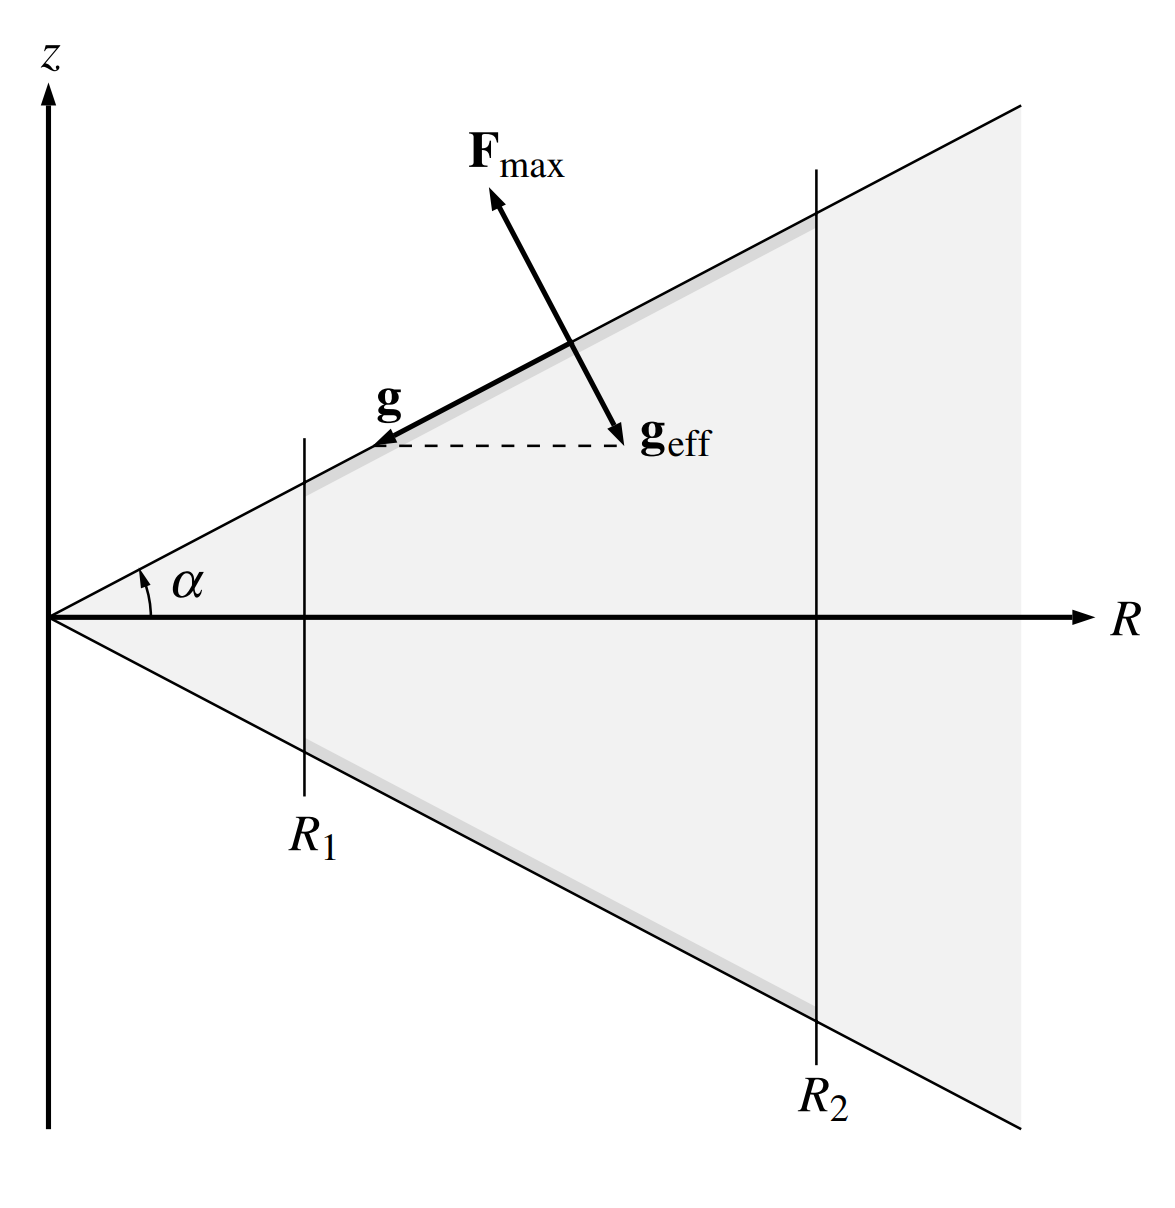
\includegraphics[width=\linewidth]{simple_geometry_geff_Lmax.png}
\caption{Effective surface gravity (rotation and gravity) balance with radiative flux to support the Keplerian rotating thick disk as in Figure \ref{fig:thick-disk-tori-struct} }\label{fig:simple_geometry_geff_Lmax}
\end{figure}
%
We will now work out the maximum luminosity that can be emitted between two radii $R_1$ and $R_2$. We can achieve this with a direct integration of $F_{max}$ on both sides of the disk
\begin{equation}
    L_{max}=2\int_{R_1}^{R_2} F_{max} (2\pi R/\cos\alpha) dR .
\end{equation}
We can evaluate the integral using \ref{eq:angular_velocity} and \ref{eq:Fmax-rad} or directly by using simple geometry see Figure \ref{fig:simple_geometry_geff_Lmax}
\begin{equation}
    F_{max}=\frac{c}{\kappa} g_{\rm{eff}} = \frac{c}{\kappa}g\tan\alpha,
\end{equation}
where $g=GM/r^2$ is the gravitational acceleration and $R=r\cos\alpha$.
This gives the result
\begin{equation} \label{eq:L_max_exceed_L_eddingtion_R1R2}
    L_{max}=L_{\rm{Edd}}\sin\alpha \ln (R_2/R_1).
\end{equation}
From \ref{eq:L_max_exceed_L_eddingtion_R1R2} it is clear that $L_{max}$ can significantly exceed $L_{\rm{Edd}}$ if $R_2/R_1$ is large. 

To summarize, in this appendix we introduced a simple thick disk. Although it is unrealistic, it does include main physical phenomena relevant to a realistic thick disk as we assume appears in nature (i.e. AGNs, YSOs, and products of stellar mergers).
In this research proposal we shall use computer simulations to produce more realistic thick disks and examine whether they can produce the main observation features.

%\hrulefill

\newpage
%\bibliographystyle{plain}
\bibliography{db}

\end{document}
